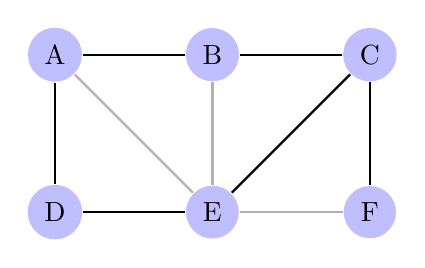
\begin{tikzpicture}
[auto,thick,node distance=2cm,every node/.style={circle,fill=blue!25}]
	\node (D) {D};
  \node (A) [above of=D] {A};
  \node (E) [right of=D] {E};
  \node (B) [right of=A] {B};
  \node (F) [right of=E] {F};
  \node (C) [right of=B] {C};

	\path
	(F) edge (C) (C) edge (B) (B) edge (A) (A) edge (D) (D) edge (E) (E) edge (C);

	\path[black!30]
	(E) edge (A)
	    edge (B)
	(F) edge (E);
\end{tikzpicture}
